% This file is the inbox for the lecture in progress. Type today's raw notes straight into
% it: it is \input from the chapter file, so the Overleaf preview builds them live. Once the
% material has been placed into the sections, /integrate empties the file again and leaves
% this header behind. Do not delete the file or its \input line.

\begin{boxdefinition}[$\lambda$-Tree]
    Let $\lambda$ be an infinite cardinal and $\parenth{T, <_T}$ be a tree. Then $T$ is a \textbf{$\lambda$-tree} iff $T$ has height $\lambda$ and $\forall \alpha < \lambda$, $\abs{\level_{\alpha}\of{T}} < \lambda$.
\end{boxdefinition}

The question is whether such a tree must have a branch running all the way up.

\begin{boxdefinition}[Tree Property]
    $\lambda$ has the \textbf{tree property} (often abbreviated TP) if every normal $\lambda$-tree has a $\lambda$-branch.
\end{boxdefinition}

The trees that witness a failure of the tree property have a name.

\begin{boxdefinition}[Aronszajn Tree]
    A \textbf{$\lambda$-Aronszajn Tree} (often abbreviated $\lambda$-A-tree) is a normal $\lambda$-tree with no $\lambda$-branch.
\end{boxdefinition}

Thus $\lambda$ has the TP iff there are no $\lambda$-A-trees. At the first two infinite cardinals, the answers go opposite ways.

\begin{boxtheorem}[K\H{o}nig]
    $\omega$ has the TP.
\end{boxtheorem}

\begin{boxtheorem}[Aronszajn]
    $\omega_1$ does \textit{not} have the TP.
\end{boxtheorem}

Proofs can be found in Ernest's book~\cite[Theorems 5.17 and 5.30]{Schimmerling} and in Kunen~\cite[Chapter II, Lemma 5.7 and Theorem 5.9]{Kunen}.

\begin{boxdefinition}[Comparability and Incomparability]
    Given a tree $T$, we say $x$ and $y$ are \textbf{comparable} (written $x \parallel y$) iff $x \leq_T y$ or $y \leq_T x$. Else, we say $x$ and $y$ are \textbf{incomparable} and write $x \perp y$.
\end{boxdefinition}

\begin{boxdefinition}[Antichain]
    $A \ssq T$ is an \textbf{antichain} (often abbreviated ac) if $\forall x, y \in A$, $x \neq y$ implies $x \perp y$.
\end{boxdefinition}

\begin{boxexample}
    For every $\alpha$, $\level_{\alpha}\of{T}$ is an antichain.
\end{boxexample}

% fill in from phone pictures

% state jensen's theorem

\begin{boxdefinition}[$\Diamond$]
    Let $\lambda$ be a regular, uncountable cardinal. Let $E \ssq \lambda$. We define \textbf{$\Diamond_{\lambda}(E)$} to be the statement that there is some sequence $\grpres{A_{\alpha}}{\alpha \in E}$ such that the following both hold:
    \begin{enumerate}
        \item Each $A_{\alpha}$ is a subset of $\alpha$
        \item For every $X \ssq \lambda$, the set $S_X = \setst{\alpha \in E}{\alpha \cap X = A_{\alpha}}$ is a stationary subset of $\lambda$.
    \end{enumerate}
    $\Diamond_{\lambda}(E)$ is shorthand the statement that there is a $\Diamond_{\lambda}(E)$-sequence, and $\Diamond_{\lambda}$ is shorthand for the statement that there is a $\Diamond_{\lambda}(\lambda)$-sequence.
\end{boxdefinition}

\begin{boxproposition}[Properties of $\Diamond$]\hfill
    \begin{enumerate}
        \item $\Diamond_{\lambda} \equiv \Diamond_{\lambda}(\lambda)$
        \item $\Diamond(E) \equiv  \Diamond_{\omega_1}(E)$
        \item $\Diamond \equiv \Diamond_{\omega_1}\of{\omega_1} = \Diamond_{\omega_1}$
    \end{enumerate}
\end{boxproposition}

\begin{boxlemma}
    Suppose $X$ is a bounded subset of $\lambda$ (so we have $\beta < \lambda$ such that $X \ssq \beta$). Assume $\grpres{A_{\alpha}}{\alpha < \lambda}$ is a $\Diamond_{\lambda}$-sequence. Then $\setst{\alpha < \lambda}{A_{\alpha} = X}$ is stationary in $\lambda$.
\end{boxlemma}

\begin{boxcorollary}
    $\Diamond_{\lambda} \to 2^{<\lambda} = \lambda$.
\end{boxcorollary}

In particular, when $\lambda = \omega_1$, we have $2^{< \omega_1} = 2^{\omega} = \omega_1$, so CH holds. In other words, diamond implies CH.

\begin{boxlemma}
    Assume $\Diamond_{\lambda}(E)$. Then $\grpres{S_X}{X \ssq \lambda}$ (where $S_X$ is defined from the witness to $\Diamond_{\lambda}(E)$) splits $E$ into $2^{\lambda}$ many almost disjoint pieces. This could mean:
    \begin{itemize}
        \item For $X \neq Y$ both subsets of $\lambda$, $S_X \cap S_Y$ is bounded in $\lambda$
        \item For $X \neq Y$ both subsets of $\lambda$, $S_X \cap S_Y$ is non-stationary in $\lambda$.
    \end{itemize}
\end{boxlemma}
\begin{proof}
    For $X \neq Y$, take $\beta = \min(X \symmdiff Y) < \lambda$. Then, for $\alpha > \beta$, $X \cap \alpha \neq Y \cap \alpha$. So we can't have $X \cap \alpha = A_{\alpha}$ and $Y \cap \alpha  = A_{\alpha}$.
\end{proof}

Recall the Solovay Splitting Theorem.

\begin{boxtheorem}[Solovay Splitting Theorem]
    Given $E \ssq \lambda$ stationary, with $\lambda = \cf(\lambda) > \omega$, we can partition $E$ into $\lambda$ many pieces, each of which is stationary.
\end{boxtheorem}

\begin{boxlemma}
    $\parenth{T, <_{T}}$ is a Souslin tree iff it's a normal $\omega_1$-tree with no uncountable antichain.
\end{boxlemma}

\begin{boxdefinition}[Maximal Antichain]
    An antichain $A \ssq T$ in a tree $T$ is \textbf{maximal} iff
    \begin{enumerate}
        \item $A$ is an antichain
        \item There's no antichain $B$ with $B \supsetneq A$
    \end{enumerate}
\end{boxdefinition}

Note: if $A $is a maximal antichain then for every $x \in T$, there's some $a \in A$ such that $a \parallel x$. Otherwise, $A \cup \set{x} = B$ would be an antichain.

\begin{boxconstruction}[Constructing a Souslin Tree from a Diamond]
    Fix a $\Diamond$-sequence $\grpres{A_{\alpha}}{\alpha < \omega_1}$. By recursion, we'll build trees $\parenth{T_{\alpha}, <_{\alpha}}$ indexed by ordinals $\alpha < \omega_1$. We'll maintain:
    \begin{enumerate}
        \item $T_{\alpha}$ is a tree of height $\alpha$
        \item $T_{\alpha}$ as a set (not as a tree) is a countable ordinal. In fact, $\alpha \leq T_{\alpha} < \omega_1$
        \item For $\alpha < \beta < \omega_1$, $T_{\alpha}$ is end-extended by $T_{\beta}$ (trees) in the ``strong sense'':
        \begin{enumerate}
            \item $<_{\alpha} \ssq <_{\beta}$
            \item for every $\eta < \alpha$, $\level_{\eta}\of{T_{\alpha}} = \level_{\eta}\of{T_{\beta}}$
        \end{enumerate}
    \end{enumerate}
    The plan is to define $\parenth{T, <_T}$ to be the union of the $\parenth{T_{\alpha}, <_{\alpha}}$s and get that $\parenth{T, <_T}$ is a Souslin-tree, but other things need to hold for this. \\

    Consider the base case
    \begin{align*}
        \parenth{T_0, <_0} = \parenth{0, \emptyset}
    \end{align*}
    Define $\parenth{T_1, <_1} := \parenth{\set{0}, \emptyset}$. We want to define $T_2$ to be the tree with root $0$ and children $1$ and $2$. Or something like that. So define
    \begin{align*}
        \parenth{T_2, <_2} := \parenth{\set{0, 1, 2}, \set{(0, 1), (0, 2)}}
    \end{align*}
    \begin{figure}[H]
        \centering
        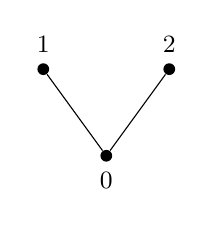
\begin{tikzpicture}[dot/.style = {circle, fill, inner sep = 1.5pt}, every node/.style = {font = \small}, grow' = up, level distance = 1.1cm, sibling distance = 1.6cm]
            \node[dot, label = {below:$0$}] {}
                child {node[dot, label = {above:$1$}] {}}
                child {node[dot, label = {above:$2$}] {}};
        \end{tikzpicture}
    \end{figure}
    In similar fashion, we define $T_3$ to be the tree extending $T_2$ with the children of $1$ being $3$ and $4$ and the children of $2$ being $5$ and $6$.
    \begin{figure}[H]
        \centering
        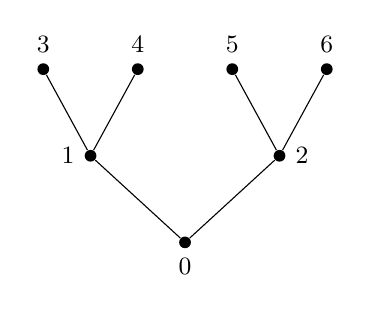
\begin{tikzpicture}[dot/.style = {circle, fill, inner sep = 1.5pt}, every node/.style = {font = \small}, grow' = up, level distance = 1.1cm, level 1/.style = {sibling distance = 2.4cm}, level 2/.style = {sibling distance = 1.2cm}]
            \node[dot, label = {below:$0$}] {}
                child {node[dot, label = {left:$1$}] {}
                    child {node[dot, label = {above:$3$}] {}}
                    child {node[dot, label = {above:$4$}] {}}}
                child {node[dot, label = {right:$2$}] {}
                    child {node[dot, label = {above:$5$}] {}}
                    child {node[dot, label = {above:$6$}] {}}};
        \end{tikzpicture}
    \end{figure}
    This is how we define successor trees. \\

    % Transcribed from the board photographs.
    % [CORRECTED] was: ``can be listed as $\xi_n$ for $n < \omega$'' and ``is $T_{\gamma} + \omega$'', for every $\beta$ --- when $\beta$ is finite the level has $2^{\beta}$ nodes and $T_{\delta} = T_{\gamma} + 2^{\beta + 1}$ (eg $T_3 = 7$, not $\omega$)
    Now consider the successor of a successor level. Say $\delta = \gamma + 1 = \parenth{\beta + 1} + 1$. How do we define $\parenth{T_{\delta}, <_{\delta}}$ based on $\parenth{T_{\gamma}, <_{\gamma}}$? We know (by the recursion hypothesis) that the universe of $T_{\gamma}$ is a countable ordinal. So $\level_{\beta}\of{T_{\gamma}}$ can be listed as $\xi_n$ for $n < \omega$ (for $n < 2^{\beta}$, if $\beta$ is finite). Define $T_{\delta}$ by putting $T_{\gamma} + 2n$ and $T_{\gamma} + 2n + 1$ above $\xi_n$.
    \begin{figure}[H]
        \centering
        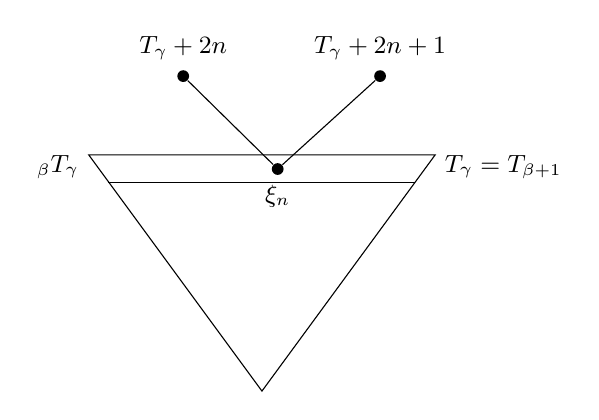
\begin{tikzpicture}[dot/.style = {circle, fill, inner sep = 1.5pt}, every node/.style = {font = \small}]
            \draw (0, 0) -- (-2.2, 3) -- (2.2, 3) -- cycle;
            \draw (-1.95, 2.65) -- (1.95, 2.65);
            \node[left] at (-2.2, 2.85) {$\level_{\beta}\of{T_{\gamma}}$};
            \node[right] at (2.2, 2.85) {$T_{\gamma} = T_{\beta + 1}$};
            \node[dot, label = {below:$\xi_n$}] (x) at (0.2, 2.82) {};
            \node[dot, label = {above:$T_{\gamma} + 2n$}] (y) at (-1, 4) {};
            \node[dot, label = {above:$T_{\gamma} + 2n + 1$}] (z) at (1.5, 4) {};
            \draw (x) -- (y);
            \draw (x) -- (z);
        \end{tikzpicture}
    \end{figure}
    We see that $T_{\delta}$ (the universe) is $T_{\gamma} + \omega$ (or $T_{\gamma} + 2^{\beta + 1}$, if $\beta$ is finite, as with $T_2$ and $T_3$). \\

    At every limit ordinal $\beta < \omega_1$, define
    \begin{align*}
        \parenth{T_{\beta}, <_{\beta}} := \parenth{\bigcup_{\alpha < \beta} T_{\alpha}, \bigcup_{\alpha < \beta} <_{\alpha}}
    \end{align*}
    In particular, we now know $\parenth{T_{\omega}, <_{\omega}}$. It's easy to see that $\parenth{T_{\omega}, <_{\omega}} \simeq {^{<\omega}2}$.

    % Transcribed from the board photographs.
    All that remains is
    \begin{enumerate}
        \item how to define $\parenth{T_{\delta}, <_{\delta}}$ when $\delta = \gamma + 1$ and $\gamma$ is a limit ordinal, and
        \item why it works.
    \end{enumerate}
\end{boxconstruction}